\documentclass{book}
 
%Russian-specific packages
%--------------------------------------
\usepackage[T2A]{fontenc}
\usepackage[utf8]{inputenc}
\usepackage[russian]{babel}
%--------------------------------------
 
%Hyphenation rules
%--------------------------------------
\usepackage{hyphenat}
\hyphenation{ма-те-ма-ти-ка вос-ста-нав-ли-вать}
%--------------------------------------
 
\usepackage{graphicx}
\graphicspath{{./img/}}
\begin{document}
 
\tableofcontents

\chapter[сравнение гипотез]{Что такое не везёт и как это рассчитывать : p-values и что делать, когда их много}

\section*{}
Начнём эту главу, пожалуй, с того, что баейсовский подход к вероятности позволяет нам немного посмотреть на то, как мы узнаём мир. Мы что-то знали (предполагали), потом что-то случилось, наши знания изменились. То, что было предположениями (априори) скорректировалось произошедшим событием, но для следующего наблюдения это - априори. Можно ждать следующего

\begin{figure}
    \centering
    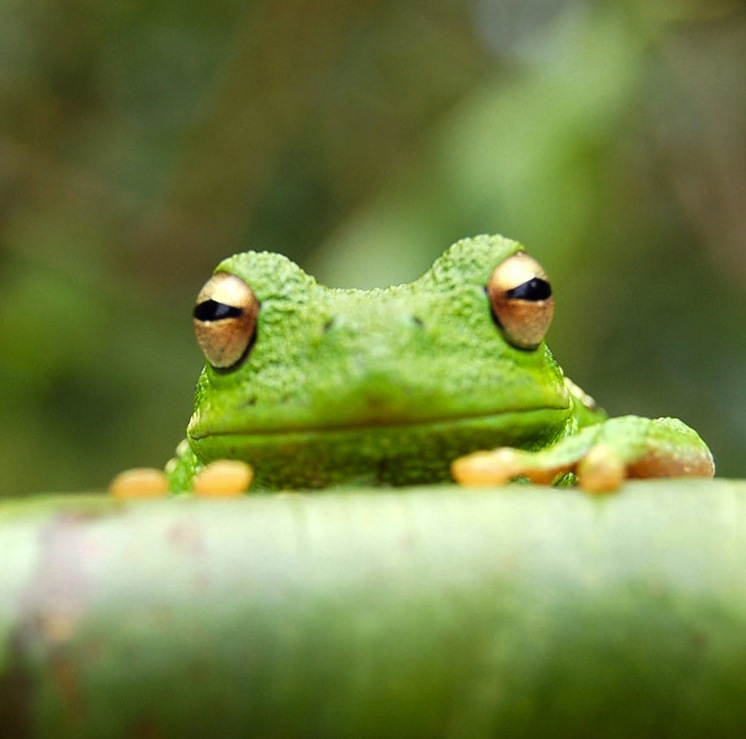
\includegraphics[scale=.5]{frog.jpg}
    \caption{Как мимолётное}
    \label{frog}
\end{figure}


\chapter[ку]{Куку}
\section{Предисловие}
Текст, использующий кириллицу, чтобы показать, что символы отображаются правильно. Вы должны установить правильные кодировку и шрифт, чтобы всё работало.
 
\section{Математические формулы}
Кириллические символы также могут быть использованы в математическом режиме.
 
\begin{equation}
  S_\textup{ис} = S_{123}
\end{equation}
 
\end{document}
